	\section{Equação do 2° Grau}

    \noindent
	\textbf{Definição}:	Uma equação linear em $x$ pode ser escrita da seguinte forma:
     \begin{tcolorbox}[colback=white,colframe=minha_cor,coltitle=black,title=Definição] 
        \begin{center}
            $ax^2+bx+c=0,$\\
		  em que $a, b, c \in \mathbb{R}$ e $a \neq 0$.
        \end{center}
        \end{tcolorbox}

    \noindent
	\textbf{Equação completa ou incompleta}\\
 
	\noindent
	\textbf{Completa} se todos os coeficientes (a, b, c) forem diferentes de 0 (zero); \\
 
	\noindent
	\textbf{Incompleta} se um dos coeficientes, b ou c, forem iguais a 0 (zero) e $a \neq 0$.

    \begin{texample}
        \centering
        \tcbhighmath{x^2+2x-3=0 \;\;\;\;\;\;\; \longrightarrow \;\;\;\; a=1, b=2; c=-3 \;\;\;\;\;\;\text{(equação completa);}}
        \tcbhighmath{-x^2+4x-3=0 \;\;\;\; \longrightarrow \;\;\;\; a=-1, b=4; c=-3 \;\;\; \text{(equação completa);}}
        \tcbhighmath{2x^2+x=0 \;\;\;\;\;\;\;\;\;\;\;\;\; \longrightarrow \;\;\;\; a=2, b=1; c=0 \;\;\;\;\;\;\;\;\;\text{(equação incompleta);}}
        \tcbhighmath{x^2+3=0 \;\;\;\;\;\;\;\;\;\;\;\;\;\;\; \longrightarrow \;\;\;\; a=1, b=0; c=3 \;\;\;\;\;\;\;\;\; \text{(equação incompleta);}}
        \tcbhighmath{x^2=0 \;\;\;\;\;\;\;\;\;\;\;\;\;\;\;\;\;\;\;\;\; \longrightarrow \;\;\;\; a=1, b=0; c=0 \;\;\;\;\;\;\;\;\;\text{(equação incompleta).}}
    \end{texample}
    
    \noindent
	\textbf{Resolução das equações}
    	O objetivo de uma equação do 2° grau é encontrar os valores de $x$ que satisfazem a igualdade.
	Pela fórmula de Bhaskara:
	\[
	\Delta = b^2 - 4 \cdot a \cdot c
	\]
	\[
	x = \dfrac{-b \pm \sqrt{ \Delta}}{2a}
	\]
	Se $\Delta > 0$, a equação tem duas raízes reais e distintas.\\
	Se $\Delta = 0$, a equação tem duas raízes reais e iguais.\\
	Se $\Delta < 0$, não existe raiz real.

    \noindent
	\textbf{Exercício resolvido}\\
	Resolva $x^2+x-6=0$\\
	Seja $a=1$, $b=1$ e $c=-6$\\
	Calculando o valor de $\Delta$
	\[
	\Delta = 1^2 - 4 \cdot 1 \cdot (-6)
	\]
	\[
	\Delta = 1 + 24
	\]
	\[
	\Delta = 25
	\]
	Como o valor de $\Delta$ é maior que 0 (zero) sabemos que a equação $x^2+x-6=0$ possui duas raízes reais e distintas. Assim,
	\[
	x = \dfrac{-1 \pm \sqrt{25}}{2 \cdot 1}
	\]
	\[
	x = \dfrac{-1 \pm 5}{2}\\
	\]
	O sinal $\pm$ na fórmula indica que devemos fazer as duas operações matemáticas (soma e subtração), sendo  $x_1$ o resultado obtido com a operação da soma (+) e $x_2$ o resultado obtido com a operação da subtração (-).\\
	Assim, em $x_1$ tem-se:
	\[
	x_1 = \dfrac{-1 + 5}{2}\\
	\]
	\[
	x_1 = \dfrac{4}{2}\\
	\]
	\[
	x_1 = 2\\
	\]
	E em $x_2$ tem-se:
	\[
	x_2 = \dfrac{-1 - 5}{2}\\
	\]
	\[
	x_2 = \dfrac{-6}{2}\\
	\]
	\[
	x_2 = -3\\
	\]
	
	O método de Bhaskara resolve todas as equações de 2º grau, porém há outras formas de resolvê-las caso verifique que a equação se enquadre em um dos casos seguintes
	\begin{description}
		\item[1º Caso:] Equações incompletas do tipo $ax^2 - c =0$ (ou seja, $b = 0$). Para resolver esse tipo de equação basta isolar a variável $x$:
		\[
		ax^2 - c =0
		\]
		\[
		ax^2 = c
		\]
		\[
		x^2 = \dfrac{c}{a}
		\]
		\[
		x = \pm \sqrt{\frac{c}{a}}
		\]
  
        \begin{texample}
        \centering
        \tcbhighmath{
            \begin{minipage}{2.5cm}
                \vspace{-0.5cm}
                \[
		      x^2 - 9 =0
		      \]
		      \[
		      x^2 = 9
		      \]
		      \[
		      x = \pm \sqrt{9}
		      \]
		      \[
		      x = \pm 3
		      \]
            \end{minipage}
        }
        \end{texample}
		
		\item[2º Caso] Equações incompletas do tipo $ax^2 + bx = 0$ (ou seja, $c=0$). Para esse caso de equação, será usada a fatoração e a incógnita $x$ é colocada em evidência, obtendo: 
		\[
		x(ax+b)=0
		\]
		Daí obtém-se
		\[
		x=0 \;\;\text{ou} \;\;ax + b=0
		\]
		\[
		ax=-b
		\]
		\[
		x=\dfrac{-b}{a}
		\]
		Então as raízes da equação são $x_1 = 0$ e $x_2 = - \dfrac{b}{a}$\\

        \begin{texample}
        \centering
        \tcbhighmath{
            \begin{minipage}{8cm}
                \[
		      x^2-5x=0
		      \]
		      Fatorando, obtém-se:
		      \[
		      x(x-5)=0
		      \]
		      Para resultar em zero um dos fatores tem que ser zero. Deste modo:
		      \[
		      x_1=0 \;\; \text{ou} \;\; x-5=0 \longrightarrow x_2=5
		      \]
            \end{minipage}
        }
        \end{texample}
		
		\item[3º Caso] Equações incompletas do tipo $ax^2 = 0$ (ou seja, $b=0$ e $c=0$). Nesse caso, as etapas são as seguintes:
		\[
		ax^2 = 0
		\]
		\[
		x^2 = \dfrac{0}{a}
		\]
		\[
		x^2 = 0
		\]
		\[
		x = 0
		\]
		Como $+0$ e $-0$ indicam o mesmo número pode-se afirmar que esse tipo de equação tem sempre duas raízes iguais a zero.
		
		\item[4º Caso] Nas equações completas podemos utilizar o método das relações de \textbf{Soma e produto} entre as raízes da equação (\textbf{relação de Girard}).
		
		\[
		x_1 + x_2 = - \dfrac{b}{a}
		\]
		\[
		x_1\; \cdot \; x_2 = \dfrac{c}{a}
		\]

        \begin{texample}
        \centering
        \tcbhighmath{
            \begin{minipage}{10cm}
                \[
		      x^2-5x+6
		      \]
		      Pela relação da Soma\\
		      \[
		      x_1 + x_2 = - \dfrac{b}{a} = - \dfrac{(-5)}{1} = 5
		      \]
		      Na relação do Produto, temos:\\
		      \[
		      x_1 \cdot x_2 = \dfrac{c}{a} = \dfrac{(6)}{1} = 6
		      \]
                Em seguida, devemos perguntar: ``quais dois números cuja soma a soma é igual a 5 e o produto é igual a 6?''\\
		      A solução é $S = \{2, 3\}$  
            \end{minipage}
        }
        \end{texample}
	\end{description}
	
	\section{Inequação do 2º Grau}
 
	\noindent
	\textbf{Definição:}	A inequação é uma desigualdade, logo em vez de um sinal de igual na sentença matemática utiliza-se sinais como:\\
	
	\begin{table}[htbp]
		\centering
		\caption{Símbolos de uma inequação.}
		\begin{tabular}{cc}
			\hline
			Símbolo &  Significado \bigstrut\\
			\hline
			<  & Menor que \bigstrut\\
			> & Maior que \bigstrut\\
			$\le$ &  Menor que ou igual a \bigstrut\\
			$\ge$ &  Maior que ou igual a \\
            \hline
		\end{tabular}%
		\label{tab:addlabel}%
	\end{table}%
	Assim, uma inequação é escrita na forma: $ax^2 + bx + c \; \Box \; 0$, em que $a, b, c \in \mathbb{R} \text{ e } a \neq 0$\\
 
	Por exemplo, na desigualdade $x^2 + 6x + 9 > 0$, tem se:
	
	\begin{table}[htbp]
		\centering
		\caption{Termos da inequação.}
		\begin{tabular}{cc}
			\hline
			Nome &  Termo \bigstrut\\
			\hline
			Incógnita  & $x$ (o maior expoente de $x$ é igual a $2$) \bigstrut\\
			1º membro & $x^2 + 6x + 9$ \bigstrut\\
			2º membro &  $0$ \\
            \hline
		\end{tabular}%
		\label{tab:addlabel}%
	\end{table}%
 
	\noindent
	\textbf{Observação:} Resolver a inequação é encontrar todos os valores reais  de $x$ que tornem a desigualdade verdadeira e escrever o conjunto solução.\\
    \noindent
	\textbf{Exercícios resolvidos.}\\
	Resolva as inequações:
	\begin{tasks}
		\task $y = x^2 - 2x -8 < 0$\\
		Resolução:\\
		Seja $a=1, b=-2, c=-8$:\\
		Encontrando o valor de $\Delta$
		\[
		\Delta = b^2 - 4 \cdot a \cdot c
		\]
		\[
		\Delta = (-2)^2 - 4 \cdot 1 \cdot (-8)
		\]
		\[
		\Delta = 4 + 32
		\]
		\[
		\Delta = 36 > 0 \longrightarrow (x_1 \neq x_2)
		\]
		Calculando os valores das raízes
		\[
		x = \dfrac{-b \pm \sqrt{ \Delta}}{2a}
		\]
		\[
		x = \dfrac{2 \pm \sqrt{36}}{2 \cdot 1}
		\]
		\[
		x = \dfrac{2 \pm 6}{2}\\
		\]
		\[
		x_1 = \dfrac{2 + 6}{2} = \dfrac{8}{2} = 4\\
		\] 
		\[
		x_2 = \dfrac{2 - 6}{2} = \dfrac{-4}{2} = -2\\
		\]   
		  %%%%%%%%%%%%%%%%%%%%%%%%%%%%%%%%%%%%%%
    \begin{center}
        \begin{tikzpicture}
            \begin{axis}[
            width=0.8\textwidth,
            xlabel=$x$,
            ylabel=$y$,
            axis lines=middle,
            xmin=-6,
            xmax=6,
            ymin=-10,
            ymax=10,
            xtick={-6,-5,...,6},
            ytick={-10,-8,...,10},
            enlargelimits,
            ticks=both,
            %tick label style={font=\small}, % para diminuir o tamanho de fonte
            tick label style={font=\footnotesize}, % outra opção de tamanho de fonte
            % tick label style={font=\tiny} % é a menor fonte q tem
            after end axis/.code={
            \draw (axis cs:0,\pgfkeysvalueof{/pgfplots/ymin}) -- (axis cs:0,\pgfkeysvalueof{/pgfplots/ymax});
            \draw (axis cs:\pgfkeysvalueof{/pgfplots/xmin},0) -- (axis cs:\pgfkeysvalueof{/pgfplots/xmax},0);
            \node[black, above right] at (axis cs:0.9,6) {$y=x^2-2x-8$};
            }
            ]
            \addplot[domain=-6:6, blue, samples=100] {x^2-2*x-8};
            \end{axis}
            \end{tikzpicture}
    \end{center}
            %%%%%%%%%%%%%%%%%%%%%%%%%%%%%%%%%%%%%%

            
		Assim, o conjunto solução é: $  S=\{ x \in \mathbb{R} \mid -2 < x < 4 \} $\\
		
		\task $-x^2 - 3x -2 \le 0$\\
		Resolução:\\
		Seja $a=-1, b=-3, c=-2$:\\
		Encontrando o valor de $\Delta$
		\[
		\Delta = b^2 - 4 \cdot a \cdot c
		\]
		\[
		\Delta = (-3)^2 - 4 \cdot (-1) \cdot (-2)
		\]
		\[
		\Delta = 9 - 8
		\]
		\[
		\Delta = 1 > 0 \longrightarrow (x_1 \neq x_2)
		\]
		Calculando os valores das raízes
		\[
		x = \dfrac{-b \pm \sqrt{ \Delta}}{2a}
		\]
		\[
		x = \dfrac{-(-3) \pm \sqrt{1}}{2 \cdot (-1)}
		\]
		\[
		x = - \dfrac{3 \pm 1}{2}\\
		\]
		\[
		x_1 = - \dfrac{3 + 1}{2} = - \dfrac{4}{2} = -2\\
		\] 
		\[
		x_2 = - \dfrac{3 - 1}{2} = - \dfrac{2}{2} = -1\\
		\]   

  
		  %%%%%%%%%%%%%%%%%%%%%%%%%%%%%%%%%%%%%%	
    \begin{center}
		  \begin{tikzpicture}
            \begin{axis}[
            width=0.8\textwidth,
            xlabel=$x$,
            ylabel=$y$,
            axis lines=middle,
            xmin=-4,
            xmax=3,
            ymin=-6,
            ymax=2,
            xtick={-4,-3,...,3},
            ytick={-6,-4,...,2},
            enlargelimits,
            ticks=both,
            %tick label style={font=\small}, % para diminuir o tamanho de fonte
            tick label style={font=\footnotesize}, % outra opção de tamanho de fonte
            % tick label style={font=\tiny} % é a menor fonte q tem
            after end axis/.code={
            \draw (axis cs:0,\pgfkeysvalueof{/pgfplots/ymin}) -- (axis cs:0,\pgfkeysvalueof{/pgfplots/ymax});
            \draw (axis cs:\pgfkeysvalueof{/pgfplots/xmin},0) -- (axis cs:\pgfkeysvalueof{/pgfplots/xmax},0);
            \node[black, above right] at (axis cs:0.5,-4) {$y=-x^2-3x-2$};
            }
            ]
            \addplot[domain=-5:3, blue, samples=100] {-x^2-3*x-2};
            \end{axis}
            \end{tikzpicture}
    \end{center}
            %%%%%%%%%%%%%%%%%%%%%%%%%%%%%%%%%%%%%%
            
            
		Assim, o conjunto solução é: $  S=\{ x \in \mathbb{R} \mid x \le -2 \text{ ou } x \ge -1 \} $
		
		\task $2x^2 - 2x +5 > 0$\\
		Resolução:\\
		Seja $a=2, b=-2, c=5$:\\
		Encontrando o valor de $\Delta$
		\[
		\Delta = b^2 - 4 \cdot a \cdot c
		\]
		\[
		\Delta = (-2)^2 - 4 \cdot 2 \cdot 5
		\]
		\[
		\Delta = 4 - 40
		\]
		\[
		\Delta = -36 < 0 \longrightarrow (x_1\; \text{e}\; x_2 \notin \mathbb{R} )
		\]
            %%%%%%%%%%%%%%%%%%%%%%%%%%%%%%%%%%%%%%	
        \begin{center}
		  \begin{tikzpicture}
            \begin{axis}[
            width=0.8\textwidth,
            xlabel=$x$,
            ylabel=$y$,
            axis lines=middle,
            xmin=-2,
            xmax=3,
            ymin=0,
            ymax=15,
            xtick={-2,-1,...,3},
            ytick={0,5,...,15},
            enlargelimits,
            ticks=both,
            %tick label style={font=\small}, % para diminuir o tamanho de fonte
            tick label style={font=\footnotesize}, % outra opção de tamanho de fonte
            % tick label style={font=\tiny} % é a menor fonte q tem
            after end axis/.code={
            \draw (axis cs:0,\pgfkeysvalueof{/pgfplots/ymin}) -- (axis cs:0,\pgfkeysvalueof{/pgfplots/ymax});
            \draw (axis cs:\pgfkeysvalueof{/pgfplots/xmin},0) -- (axis cs:\pgfkeysvalueof{/pgfplots/xmax},0);
            \node[black, above right] at (axis cs:1,10) {$y=2x^2-2x+5$};
            }
            ]
            \addplot[domain=-2:3, blue, samples=100] {2*x^2-2*x+5};
            \end{axis}
        \end{tikzpicture}
    \end{center}
            %%%%%%%%%%%%%%%%%%%%%%%%%%%%%%%%%%%%%%
            
		Assim, o conjunto solução é: $  S= \mathbb{R}$
	\end{tasks}
 
	\noindent
	\textbf{Sistemas de Inequações do 2º Grau}\\
	Existem sistemas de inequações que aparecem duas ou mais inequações do segundo grau.\\
	
	A resolução deve ser feita da seguinte forma:
	\begin{itemize}
		\item Resolver cada inequação separadamente;
		\item Fazer a intersecção das soluções usando as retas dos intervalos;
		\item Dar a solução.
	\end{itemize}

    \noindent
	\textbf{Exercício resolvido}\\

	Encontre o conjunto solução do seguinte sistema de inequações:
	
	\[ \left\{  
	\begin{array}{c}
		x^2 - 6x + 9 \ge 0\\
		3x - 6 > 0\\
	\end{array} 
	\right.
	\]
	\noindent
	Resolução:\\
	\begin{flushleft}
		$
		\left\{  
		\begin{array}{c}
			x^2 - 6x + 9 \ge 0 \;\;\;\; \text{Inequação (I)}\\
			3x - 6 > 0 \;\;\;\;\;\;\;\;\;\;\;\;\: \text{Inequação (II)}\\
		\end{array} 
		\right.
		$
	\end{flushleft}
	Resolvendo separadamente a inequação (I), temos:\\
	$ x^2 - 6x + 9 \ge 0$\\
	Seja $a=1, b=-6, c=9$:\\
	\[
	\Delta = b^2 - 4 \cdot a \cdot c
	\]
	\[
	\Delta = (-6)^2 - 4 \cdot 1 \cdot 9
	\]
	\[
	\Delta = 0 \longrightarrow (x_1 = x_2)
	\]
	Calculando os valores das raízes
	\[
	x = \dfrac{-b \pm \sqrt{ \Delta}}{2a}
	\]
	\[
	x = \dfrac{-(-6) \pm \sqrt{0}}{2 \cdot 1}
	\]
	\[
	x = \dfrac{6 \pm 0}{2} =\dfrac{6}{2}\longrightarrow x_1 = x_2 = 3\\
	\]
	
	       %%%%%%%%%%%%%%%%%%%%%%%%%%%%%%%%%%%%%%	
        \begin{center}
		  \begin{tikzpicture}
            \begin{axis}[
            width=0.8\textwidth,
            xlabel=$x$,
            ylabel=$y$,
            axis lines=middle,
            xmin=-2,
            xmax=10,
            ymin=0,
            ymax=10,
            xtick={-2,0,...,10},
            ytick={0,2,...,10},
            enlargelimits,
            ticks=both,
            %tick label style={font=\small}, % para diminuir o tamanho de fonte
            tick label style={font=\footnotesize}, % outra opção de tamanho de fonte
            % tick label style={font=\tiny} % é a menor fonte q tem
            after end axis/.code={
            \draw (axis cs:0,\pgfkeysvalueof{/pgfplots/ymin}) -- (axis cs:0,\pgfkeysvalueof{/pgfplots/ymax});
            \draw (axis cs:\pgfkeysvalueof{/pgfplots/xmin},0) -- (axis cs:\pgfkeysvalueof{/pgfplots/xmax},0);
            \node[black, above right] at (axis cs:4.6,2) {$y=x^2-6x+9$};
            }
            ]
            \addplot[domain=-2:10, blue, samples=100] {x^2-6*x+9};
            \end{axis}
        \end{tikzpicture}
    \end{center}
            %%%%%%%%%%%%%%%%%%%%%%%%%%%%%%%%%%%%%%
	
	O conjunto solução da Inequação (I) é: $  S_1 = \mathbb{R}  $\\
	
	Resolvendo separadamente a inequação (I), temos:\\
	\[ 3x -6 > 0 \]
	\[ 3x - 6 = 0 \]
	\[ 3x = 6\]
	\[ x = \dfrac{6}{3} = 2 \]

         %%%%%%%%%%%%%%%%%%%%%%%%%%%%%%%%%%%%%%	
        \begin{center}
		  \begin{tikzpicture}
            \begin{axis}[
            width=0.8\textwidth,
            xlabel=$x$,
            ylabel=$y$,
            axis lines=middle,
            xmin=-2,
            xmax=6,
            ymin=-6,
            ymax=6,
            xtick={-2,-1,...,6},
            ytick={-6,4,...,6},
            enlargelimits,
            ticks=both,
            %tick label style={font=\small}, % para diminuir o tamanho de fonte
            tick label style={font=\footnotesize}, % outra opção de tamanho de fonte
            % tick label style={font=\tiny} % é a menor fonte q tem
            after end axis/.code={
            \draw (axis cs:0,\pgfkeysvalueof{/pgfplots/ymin}) -- (axis cs:0,\pgfkeysvalueof{/pgfplots/ymax});
            \draw (axis cs:\pgfkeysvalueof{/pgfplots/xmin},0) -- (axis cs:\pgfkeysvalueof{/pgfplots/xmax},0);
            \node[black, above right] at (axis cs:3,2) {$y=3x-6$};
            }
            ]
            \addplot[domain=-2:6, blue, samples=100] {3*x-6};
            \end{axis}
        \end{tikzpicture}
    \end{center}
            %%%%%%%%%%%%%%%%%%%%%%%%%%%%%%%%%%%%%%
	
	O conjunto solução da Inequação (II) é: $  S_2 = \{ x \in \mathbb{R} \mid x > 2 \} $.       
 
%%%%%%%%%%%%%%%%%%%%%%%%%%%%%%%%%%%%%%%%%%%%%%%%%%%%%%%
     
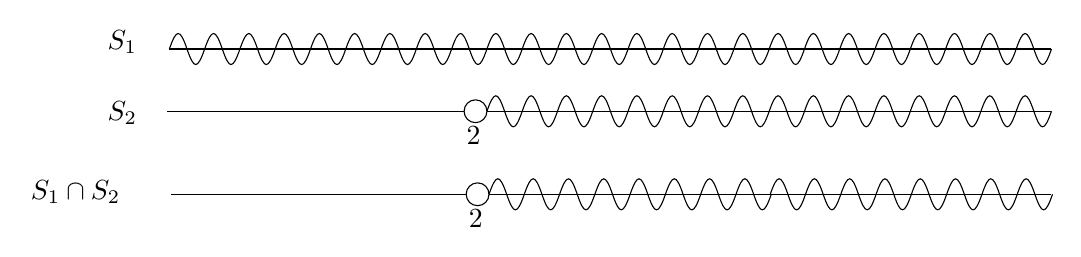
\begin{tikzpicture}[x=0.75pt,y=0.75pt,yscale=-1,xscale=1]

\draw [color={rgb, 255:red, 0; green, 0; blue, 0 }  ,draw opacity=1 ]   (107,140) -- (249,140) ;
%Shape: Circle [id:dp499328118003723] 
\draw   (249,140) .. controls (249,136.96) and (251.46,134.5) .. (254.5,134.5) .. controls (257.54,134.5) and (260,136.96) .. (260,140) .. controls (260,143.04) and (257.54,145.5) .. (254.5,145.5) .. controls (251.46,145.5) and (249,143.04) .. (249,140) -- cycle ;
%Straight Lines [id:da983248389983719] 
\draw [color={rgb, 255:red, 0; green, 0; blue, 0 }  ,draw opacity=1 ]   (260,140) -- (531,140) ;
%Shape: Sine Wave Form [id:dp19261270162193456] 
\draw   (260,140) .. controls (263.46,130.08) and (265.09,130.03) .. (268.5,140) .. controls (271.91,149.97) and (273.51,150.03) .. (277,140) ;
%Shape: Sine Wave Form [id:dp9956746811450048] 
\draw   (277,140) .. controls (280.46,130.08) and (282.09,130.03) .. (285.5,140) .. controls (288.91,149.97) and (290.51,150.03) .. (294,140) ;
%Shape: Sine Wave Form [id:dp49013479930459414] 
\draw   (294,140) .. controls (297.46,130.08) and (299.09,130.03) .. (302.5,140) .. controls (305.91,149.97) and (307.51,150.03) .. (311,140) ;
%Shape: Sine Wave Form [id:dp8997338292124744] 
\draw   (311,140) .. controls (314.46,130.08) and (316.09,130.03) .. (319.5,140) .. controls (322.91,149.97) and (324.51,150.03) .. (328,140) ;
%Shape: Sine Wave Form [id:dp9547555964802317] 
\draw   (328,140) .. controls (331.46,130.08) and (333.09,130.03) .. (336.5,140) .. controls (339.91,149.97) and (341.51,150.03) .. (345,140) ;
%Shape: Sine Wave Form [id:dp43280309296471686] 
\draw   (345,140) .. controls (348.46,130.08) and (350.09,130.03) .. (353.5,140) .. controls (356.91,149.97) and (358.51,150.03) .. (362,140) ;
%Shape: Sine Wave Form [id:dp7293692976551054] 
\draw   (362,140) .. controls (365.46,130.08) and (367.09,130.03) .. (370.5,140) .. controls (373.91,149.97) and (375.51,150.03) .. (379,140) ;
%Shape: Sine Wave Form [id:dp5139065198397219] 
\draw   (379,140) .. controls (382.46,130.08) and (384.09,130.03) .. (387.5,140) .. controls (390.91,149.97) and (392.51,150.03) .. (396,140) ;
%Shape: Sine Wave Form [id:dp8865955899516669] 
\draw   (395.5,140) .. controls (398.96,130.08) and (400.59,130.03) .. (404,140) .. controls (407.41,149.97) and (409.01,150.03) .. (412.5,140) ;
%Shape: Sine Wave Form [id:dp08625524836758869] 
\draw   (412.5,140) .. controls (415.96,130.08) and (417.59,130.03) .. (421,140) .. controls (424.41,149.97) and (426.01,150.03) .. (429.5,140) ;
%Shape: Sine Wave Form [id:dp6712584938884274] 
\draw   (429.5,140) .. controls (432.96,130.08) and (434.59,130.03) .. (438,140) .. controls (441.41,149.97) and (443.01,150.03) .. (446.5,140) ;
%Shape: Sine Wave Form [id:dp44814226752060193] 
\draw   (446.5,140) .. controls (449.96,130.08) and (451.59,130.03) .. (455,140) .. controls (458.41,149.97) and (460.01,150.03) .. (463.5,140) ;
%Shape: Sine Wave Form [id:dp0009337483565319271] 
\draw   (463.5,140) .. controls (466.96,130.08) and (468.59,130.03) .. (472,140) .. controls (475.41,149.97) and (477.01,150.03) .. (480.5,140) ;
%Shape: Sine Wave Form [id:dp54985570827407] 
\draw   (480.5,140) .. controls (483.96,130.08) and (485.59,130.03) .. (489,140) .. controls (492.41,149.97) and (494.01,150.03) .. (497.5,140) ;
%Shape: Sine Wave Form [id:dp2100943422373256] 
\draw   (497.5,140) .. controls (500.96,130.08) and (502.59,130.03) .. (506,140) .. controls (509.41,149.97) and (511.01,150.03) .. (514.5,140) ;
%Shape: Sine Wave Form [id:dp20925171030698042] 
\draw   (514.5,140) .. controls (517.96,130.08) and (519.59,130.03) .. (523,140) .. controls (526.41,149.97) and (528.01,150.03) .. (531.5,140) ;
%Straight Lines [id:da727970159695563] 
\draw [color={rgb, 255:red, 0; green, 0; blue, 0 }  ,draw opacity=1 ]   (105,100) -- (248,100) ;
%Shape: Circle [id:dp689038796926821] 
\draw   (248,100) .. controls (248,96.96) and (250.46,94.5) .. (253.5,94.5) .. controls (256.54,94.5) and (259,96.96) .. (259,100) .. controls (259,103.04) and (256.54,105.5) .. (253.5,105.5) .. controls (250.46,105.5) and (248,103.04) .. (248,100) -- cycle ;
%Straight Lines [id:da33391134406641965] 
\draw [color={rgb, 255:red, 0; green, 0; blue, 0 }  ,draw opacity=1 ]   (259,100) -- (531,100) ;
%Shape: Sine Wave Form [id:dp0055980554048127296] 
\draw   (259,100) .. controls (262.46,90.08) and (264.09,90.03) .. (267.5,100) .. controls (270.91,109.97) and (272.51,110.03) .. (276,100) ;
%Shape: Sine Wave Form [id:dp9460515557542251] 
\draw   (276,100) .. controls (279.46,90.08) and (281.09,90.03) .. (284.5,100) .. controls (287.91,109.97) and (289.51,110.03) .. (293,100) ;
%Shape: Sine Wave Form [id:dp8403195311582816] 
\draw   (293,100) .. controls (296.46,90.08) and (298.09,90.03) .. (301.5,100) .. controls (304.91,109.97) and (306.51,110.03) .. (310,100) ;
%Shape: Sine Wave Form [id:dp44358567364093227] 
\draw   (310,100) .. controls (313.46,90.08) and (315.09,90.03) .. (318.5,100) .. controls (321.91,109.97) and (323.51,110.03) .. (327,100) ;
%Shape: Sine Wave Form [id:dp6888464795367184] 
\draw   (327,100) .. controls (330.46,90.08) and (332.09,90.03) .. (335.5,100) .. controls (338.91,109.97) and (340.51,110.03) .. (344,100) ;
%Shape: Sine Wave Form [id:dp2233780589772869] 
\draw   (344,100) .. controls (347.46,90.08) and (349.09,90.03) .. (352.5,100) .. controls (355.91,109.97) and (357.51,110.03) .. (361,100) ;
%Shape: Sine Wave Form [id:dp7573635916153589] 
\draw   (361,100) .. controls (364.46,90.08) and (366.09,90.03) .. (369.5,100) .. controls (372.91,109.97) and (374.51,110.03) .. (378,100) ;
%Shape: Sine Wave Form [id:dp7570361164411796] 
\draw   (378,100) .. controls (381.46,90.08) and (383.09,90.03) .. (386.5,100) .. controls (389.91,109.97) and (391.51,110.03) .. (395,100) ;
%Shape: Sine Wave Form [id:dp28404239220351934] 
\draw   (395,100) .. controls (398.46,90.08) and (400.09,90.03) .. (403.5,100) .. controls (406.91,109.97) and (408.51,110.03) .. (412,100) ;
%Shape: Sine Wave Form [id:dp6584296384617263] 
\draw   (412,100) .. controls (415.46,90.08) and (417.09,90.03) .. (420.5,100) .. controls (423.91,109.97) and (425.51,110.03) .. (429,100) ;
%Shape: Sine Wave Form [id:dp7453614915314855] 
\draw   (429,100) .. controls (432.46,90.08) and (434.09,90.03) .. (437.5,100) .. controls (440.91,109.97) and (442.51,110.03) .. (446,100) ;
%Shape: Sine Wave Form [id:dp2078823016074105] 
\draw   (446,100) .. controls (449.46,90.08) and (451.09,90.03) .. (454.5,100) .. controls (457.91,109.97) and (459.51,110.03) .. (463,100) ;
%Shape: Sine Wave Form [id:dp17250855630485007] 
\draw   (463,100) .. controls (466.46,90.08) and (468.09,90.03) .. (471.5,100) .. controls (474.91,109.97) and (476.51,110.03) .. (480,100) ;
%Shape: Sine Wave Form [id:dp8679818842397253] 
\draw   (480,100) .. controls (483.46,90.08) and (485.09,90.03) .. (488.5,100) .. controls (491.91,109.97) and (493.51,110.03) .. (497,100) ;
%Shape: Sine Wave Form [id:dp7723965903973888] 
\draw   (497,100) .. controls (500.46,90.08) and (502.09,90.03) .. (505.5,100) .. controls (508.91,109.97) and (510.51,110.03) .. (514,100) ;
%Shape: Sine Wave Form [id:dp6823852906218766] 
\draw   (514,100) .. controls (517.46,90.08) and (519.09,90.03) .. (522.5,100) .. controls (525.91,109.97) and (527.51,110.03) .. (531,100) ;
%Straight Lines [id:da6310652526442746] 
\draw [color={rgb, 255:red, 0; green, 0; blue, 0 }  ,draw opacity=1 ]   (106,70) -- (259,70) ;
%Straight Lines [id:da9854307779091338] 
\draw [color={rgb, 255:red, 0; green, 0; blue, 0 }  ,draw opacity=1 ]   (259,70) -- (531,70) ;
%Shape: Sine Wave Form [id:dp05380894872453856] 
\draw   (259,70) .. controls (262.46,60.08) and (264.09,60.03) .. (267.5,70) .. controls (270.91,79.97) and (272.51,80.03) .. (276,70) ;
%Shape: Sine Wave Form [id:dp9175368674925128] 
\draw   (276,70) .. controls (279.46,60.08) and (281.09,60.03) .. (284.5,70) .. controls (287.91,79.97) and (289.51,80.03) .. (293,70) ;
%Shape: Sine Wave Form [id:dp3645931158395448] 
\draw   (293,70) .. controls (296.46,60.08) and (298.09,60.03) .. (301.5,70) .. controls (304.91,79.97) and (306.51,80.03) .. (310,70) ;
%Shape: Sine Wave Form [id:dp1510743578453433] 
\draw   (310,70) .. controls (313.46,60.08) and (315.09,60.03) .. (318.5,70) .. controls (321.91,79.97) and (323.51,80.03) .. (327,70) ;
%Shape: Sine Wave Form [id:dp6634970689846824] 
\draw   (327,70) .. controls (330.46,60.08) and (332.09,60.03) .. (335.5,70) .. controls (338.91,79.97) and (340.51,80.03) .. (344,70) ;
%Shape: Sine Wave Form [id:dp173263983418098] 
\draw   (344,70) .. controls (347.46,60.08) and (349.09,60.03) .. (352.5,70) .. controls (355.91,79.97) and (357.51,80.03) .. (361,70) ;
%Shape: Sine Wave Form [id:dp9544693761739522] 
\draw   (361,70) .. controls (364.46,60.08) and (366.09,60.03) .. (369.5,70) .. controls (372.91,79.97) and (374.51,80.03) .. (378,70) ;
%Shape: Sine Wave Form [id:dp8748552836295116] 
\draw   (378,70) .. controls (381.46,60.08) and (383.09,60.03) .. (386.5,70) .. controls (389.91,79.97) and (391.51,80.03) .. (395,70) ;
%Shape: Sine Wave Form [id:dp8723947950562154] 
\draw   (395,70) .. controls (398.46,60.08) and (400.09,60.03) .. (403.5,70) .. controls (406.91,79.97) and (408.51,80.03) .. (412,70) ;
%Shape: Sine Wave Form [id:dp26039806103418783] 
\draw   (412,70) .. controls (415.46,60.08) and (417.09,60.03) .. (420.5,70) .. controls (423.91,79.97) and (425.51,80.03) .. (429,70) ;
%Shape: Sine Wave Form [id:dp9159858783285941] 
\draw   (429,70) .. controls (432.46,60.08) and (434.09,60.03) .. (437.5,70) .. controls (440.91,79.97) and (442.51,80.03) .. (446,70) ;
%Shape: Sine Wave Form [id:dp048563199455269324] 
\draw   (446,70) .. controls (449.46,60.08) and (451.09,60.03) .. (454.5,70) .. controls (457.91,79.97) and (459.51,80.03) .. (463,70) ;
%Shape: Sine Wave Form [id:dp17105636645741518] 
\draw   (463,70) .. controls (466.46,60.08) and (468.09,60.03) .. (471.5,70) .. controls (474.91,79.97) and (476.51,80.03) .. (480,70) ;
%Shape: Sine Wave Form [id:dp31960182937750314] 
\draw   (480,70) .. controls (483.46,60.08) and (485.09,60.03) .. (488.5,70) .. controls (491.91,79.97) and (493.51,80.03) .. (497,70) ;
%Shape: Sine Wave Form [id:dp24318304860610507] 
\draw   (497,70) .. controls (500.46,60.08) and (502.09,60.03) .. (505.5,70) .. controls (508.91,79.97) and (510.51,80.03) .. (514,70) ;
%Shape: Sine Wave Form [id:dp6601921052538] 
\draw   (514,70) .. controls (517.46,60.08) and (519.09,60.03) .. (522.5,70) .. controls (525.91,79.97) and (527.51,80.03) .. (531,70) ;
%Shape: Sine Wave Form [id:dp6024401907607075] 
\draw   (106,70) .. controls (109.46,60.08) and (111.09,60.03) .. (114.5,70) .. controls (117.91,79.97) and (119.51,80.03) .. (123,70) ;
%Shape: Sine Wave Form [id:dp6162493633840183] 
\draw   (123,70) .. controls (126.46,60.08) and (128.09,60.03) .. (131.5,70) .. controls (134.91,79.97) and (136.51,80.03) .. (140,70) ;
%Shape: Sine Wave Form [id:dp1894812842271716] 
\draw   (140,70) .. controls (143.46,60.08) and (145.09,60.03) .. (148.5,70) .. controls (151.91,79.97) and (153.51,80.03) .. (157,70) ;
%Shape: Sine Wave Form [id:dp5928204332014821] 
\draw   (157,70) .. controls (160.46,60.08) and (162.09,60.03) .. (165.5,70) .. controls (168.91,79.97) and (170.51,80.03) .. (174,70) ;
%Shape: Sine Wave Form [id:dp864313063213568] 
\draw   (174,70) .. controls (177.46,60.08) and (179.09,60.03) .. (182.5,70) .. controls (185.91,79.97) and (187.51,80.03) .. (191,70) ;
%Shape: Sine Wave Form [id:dp1489180832283037] 
\draw   (191,70) .. controls (194.46,60.08) and (196.09,60.03) .. (199.5,70) .. controls (202.91,79.97) and (204.51,80.03) .. (208,70) ;
%Shape: Sine Wave Form [id:dp6840095912482207] 
\draw   (208,70) .. controls (211.46,60.08) and (213.09,60.03) .. (216.5,70) .. controls (219.91,79.97) and (221.51,80.03) .. (225,70) ;
%Shape: Sine Wave Form [id:dp8769097819337193] 
\draw   (225,70) .. controls (228.46,60.08) and (230.09,60.03) .. (233.5,70) .. controls (236.91,79.97) and (238.51,80.03) .. (242,70) ;
%Shape: Sine Wave Form [id:dp5244003279828346] 
\draw   (242,70) .. controls (245.46,60.08) and (247.09,60.03) .. (250.5,70) .. controls (253.91,79.97) and (255.51,80.03) .. (259,70) ;

% Text Node
\draw (249,146) node [anchor=north west][inner sep=0.75pt]   [align=left] {2};
% Text Node
\draw (75,60) node [anchor=north west][inner sep=0.75pt]   [align=left] {$S_1$};
% Text Node
\draw (75,94) node [anchor=north west][inner sep=0.75pt]   [align=left] {$S_2$};
% Text Node
\draw (38,132) node [anchor=north west][inner sep=0.75pt]   [align=left] {$S_1 \cap S_2$};
% Text Node
\draw (248,106) node [anchor=north west][inner sep=0.75pt]   [align=left] {2};
\end{tikzpicture}

%%%%%%%%%%%%%%%%%%%%%%%%%%%%%%%%%%%%%%%%%%%%%%%%%%%%%%%
    \noindent
	\textbf{Inequações Simultâneas}\\
	
	Uma inequação do 2º grau é simultânea quando aparecer duas desigualdades numa só sentença. Sua resolução deve ser feita da mesma maneira que em sistemas de inequações do 2º grau.

    \noindent
	\textbf{Exercício resolvido.}
	
	Encontre o conjunto solução da seguinte inequação:
	\[
	3 < x^2 - 2x +8 \le 8
	\]
	
	Decompondo em um sistema de inequações, temos:
	
	\[ \left\{  
	\begin{array}{c}
		x^2 - 2x + 8 \le 8\\
		x^2 - 2x + 8 > 3\\
	\end{array} 
	\right.
	\]
	
	Em seguida, são feitas algumas manipulações necessárias para facilitar a análise e obtemos o sistema abaixo
	
	\[ \left\{  
	\begin{array}{c}
		x^2 - 2x \le 0  \;\;\;\;\;\;\;\;\;\;\;\;\;\;\text{Inequação (I)}\\
		x^2 - 2x + 5 > 0 \;\;\;\;\;\;\;\;\;\; \text{Inequação (II)}\\
	\end{array} 
	\right.
	\]
	
	Resolvendo separadamente a inequação (I), temos:\\
	$ x^2 - 2x\le 0$\\
	\[
	x^2 - 2x = 0 \;\; \longrightarrow \;\; x(x-2)
	=0\]
	\[
	\text{Assim,} \; x=0 \; \text{ou} \; x-2=0
	\]
	\[
	\text{Então, temos:} \; x_1=0 \; \text{e} \; x_2 = 2
	\]
	      %%%%%%%%%%%%%%%%%%%%%%%%%%%%%%%%%%%%%%	
        \begin{center}
		  \begin{tikzpicture}
            \begin{axis}[
            width=0.8\textwidth,
            xlabel=$x$,
            ylabel=$y$,
            axis lines=middle,
            xmin=-2,
            xmax=4,
            ymin=-2,
            ymax=8,
            xtick={-2,-1,...,4},
            ytick={-2,0,...,8},
            enlargelimits,
            ticks=both,
            %tick label style={font=\small}, % para diminuir o tamanho de fonte
            tick label style={font=\footnotesize}, % outra opção de tamanho de fonte
            % tick label style={font=\tiny} % é a menor fonte q tem
            after end axis/.code={
            \draw (axis cs:0,\pgfkeysvalueof{/pgfplots/ymin}) -- (axis cs:0,\pgfkeysvalueof{/pgfplots/ymax});
            \draw (axis cs:\pgfkeysvalueof{/pgfplots/xmin},0) -- (axis cs:\pgfkeysvalueof{/pgfplots/xmax},0);
            \node[black, above right] at (axis cs:1.9,5) {$y=x^2-2x$};
            }
            ]
            \addplot[domain=-2:4, blue, samples=100] {x^2-2*x};
            \end{axis}
        \end{tikzpicture}
    \end{center}
            %%%%%%%%%%%%%%%%%%%%%%%%%%%%%%%%%%%%%%
    O conjunto solução da Inequação I é: $  S_1 = \{ x \in \mathbb{R} \mid 0 \le x \le 2 \} $
 
    Resolvendo separadamente a inequação (II), temos:\\
	$ x^2 - 2x + 5 > 0$\\
	Seja $a=1, b=-2, c=5$:\\
	\[
	\Delta = b^2 - 4 \cdot a \cdot c
	\]
	\[
	\Delta = (-2)^2 - 4 \cdot 1 \cdot 5
	\]
	\[
	\Delta = -16 < 0 \longrightarrow (x_1 \text{ e } x_2 \notin \mathbb{R})
	\]
           %%%%%%%%%%%%%%%%%%%%%%%%%%%%%%%%%%%%%%	
        \begin{center}
		  \begin{tikzpicture}
            \begin{axis}[
            width=0.8\textwidth,
            xlabel=$x$,
            ylabel=$y$,
            axis lines=middle,
            xmin=-2,
            xmax=4,
            ymin=0,
            ymax=14,
            xtick={-2,-1,...,4},
            ytick={-2,-0,...,14},
            enlargelimits,
            ticks=both,
            %tick label style={font=\small}, % para diminuir o tamanho de fonte
            tick label style={font=\footnotesize}, % outra opção de tamanho de fonte
            % tick label style={font=\tiny} % é a menor fonte q tem
            after end axis/.code={
            \draw (axis cs:0,\pgfkeysvalueof{/pgfplots/ymin}) -- (axis cs:0,\pgfkeysvalueof{/pgfplots/ymax});
            \draw (axis cs:\pgfkeysvalueof{/pgfplots/xmin},0) -- (axis cs:\pgfkeysvalueof{/pgfplots/xmax},0);
            \node[black, above right] at (axis cs:2,4) {$y=x^2-2x+5$};
            }
            ]
            \addplot[domain=-2.2:4.2, blue, samples=100] {x^2-2*x+5};
            \end{axis}
        \end{tikzpicture}
    \end{center}
            %%%%%%%%%%%%%%%%%%%%%%%%%%%%%%%%%%%%%%
            
    O conjunto solução da Inequação I é: $  S_2 =  \mathbb{R} $.

    Assim:     
%%%%%%%%%%%%%%%%%%%%%%%%%%%%%%%%%%%%%%%%%%%%%%%%%%%%%%%%%%%%

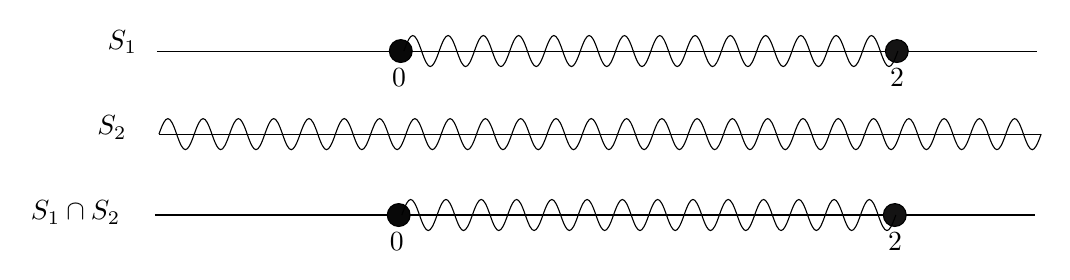
\begin{tikzpicture}[x=0.75pt,y=0.75pt,yscale=-1,xscale=1]
\draw [color={rgb, 255:red, 0; green, 0; blue, 0 }  ,draw opacity=1 ]   (99,150) -- (211,150) ;
%Shape: Circle [id:dp13394753879586196] 
\draw  [fill={rgb, 255:red, 8; green, 8; blue, 8 }  ,fill opacity=1 ] (211,150) .. controls (211,146.96) and (213.46,144.5) .. (216.5,144.5) .. controls (219.54,144.5) and (222,146.96) .. (222,150) .. controls (222,153.04) and (219.54,155.5) .. (216.5,155.5) .. controls (213.46,155.5) and (211,153.04) .. (211,150) -- cycle ;
%Shape: Circle [id:dp8140031189659684] 
\draw  [fill={rgb, 255:red, 20; green, 19; blue, 19 }  ,fill opacity=1 ] (450,150) .. controls (450,146.96) and (452.46,144.5) .. (455.5,144.5) .. controls (458.54,144.5) and (461,146.96) .. (461,150) .. controls (461,153.04) and (458.54,155.5) .. (455.5,155.5) .. controls (452.46,155.5) and (450,153.04) .. (450,150) -- cycle ;
%Straight Lines [id:da8738818381064104] 
\draw [color={rgb, 255:red, 0; green, 0; blue, 0 }  ,draw opacity=1 ]   (222,150) -- (450,150) ;
%Straight Lines [id:da2742063151206309] 
\draw [color={rgb, 255:red, 0; green, 0; blue, 0 }  ,draw opacity=1 ]   (461,150) -- (523,150) ;
%Shape: Sine Wave Form [id:dp5560135930065992] 
\draw   (218,149.97) .. controls (221.46,140.05) and (223.09,140) .. (226.5,149.97) .. controls (229.91,159.94) and (231.51,160) .. (235,149.97) ;
%Shape: Sine Wave Form [id:dp037612875437989635] 
\draw   (235,149.97) .. controls (238.46,140.05) and (240.09,140) .. (243.5,149.97) .. controls (246.91,159.94) and (248.51,160) .. (252,149.97) ;
%Shape: Sine Wave Form [id:dp607072975491741] 
\draw   (252,149.97) .. controls (255.46,140.05) and (257.09,140) .. (260.5,149.97) .. controls (263.91,159.94) and (265.51,160) .. (269,149.97) ;
%Shape: Sine Wave Form [id:dp6222363700911624] 
\draw   (269,149.97) .. controls (272.46,140.05) and (274.09,140) .. (277.5,149.97) .. controls (280.91,159.94) and (282.51,160) .. (286,149.97) ;
%Shape: Sine Wave Form [id:dp5094858474023591] 
\draw   (286,149.97) .. controls (289.46,140.05) and (291.09,140) .. (294.5,149.97) .. controls (297.91,159.94) and (299.51,160) .. (303,149.97) ;
%Shape: Sine Wave Form [id:dp14658799285941626] 
\draw   (303,149.97) .. controls (306.46,140.05) and (308.09,140) .. (311.5,149.97) .. controls (314.91,159.94) and (316.51,160) .. (320,149.97) ;
%Shape: Sine Wave Form [id:dp7509528882024004] 
\draw   (320,149.97) .. controls (323.46,140.05) and (325.09,140) .. (328.5,149.97) .. controls (331.91,159.94) and (333.51,160) .. (337,149.97) ;
%Shape: Sine Wave Form [id:dp870505599017166] 
\draw   (337,149.97) .. controls (340.46,140.05) and (342.09,140) .. (345.5,149.97) .. controls (348.91,159.94) and (350.51,160) .. (354,149.97) ;
%Shape: Sine Wave Form [id:dp38831189344034756] 
\draw   (354,149.97) .. controls (357.46,140.05) and (359.09,140) .. (362.5,149.97) .. controls (365.91,159.94) and (367.51,160) .. (371,149.97) ;
%Shape: Sine Wave Form [id:dp002785288641573347] 
\draw   (371,149.97) .. controls (374.46,140.05) and (376.09,140) .. (379.5,149.97) .. controls (382.91,159.94) and (384.51,160) .. (388,149.97) ;
%Shape: Sine Wave Form [id:dp7612226759114071] 
\draw   (388,149.97) .. controls (391.46,140.05) and (393.09,140) .. (396.5,149.97) .. controls (399.91,159.94) and (401.51,160) .. (405,149.97) ;
%Shape: Sine Wave Form [id:dp31115824624706234] 
\draw   (405,149.97) .. controls (408.46,140.05) and (410.09,140) .. (413.5,149.97) .. controls (416.91,159.94) and (418.51,160) .. (422,149.97) ;
%Shape: Sine Wave Form [id:dp686752789670718] 
\draw   (422,149.97) .. controls (425.46,140.05) and (427.09,140) .. (430.5,149.97) .. controls (433.91,159.94) and (435.51,160) .. (439,149.97) ;
%Shape: Sine Wave Form [id:dp7009231640429723] 
\draw   (439,149.97) .. controls (442.46,140.05) and (444.09,140) .. (447.5,149.97) .. controls (450.91,159.94) and (452.51,160) .. (456,149.97) ;
%Straight Lines [id:da8460748694650719] 
\draw [color={rgb, 255:red, 0; green, 0; blue, 0 }  ,draw opacity=1 ]   (101,111) -- (254,111) ;
%Straight Lines [id:da5989942174531802] 
\draw [color={rgb, 255:red, 0; green, 0; blue, 0 }  ,draw opacity=1 ]   (254,111) -- (526,111) ;
%Shape: Sine Wave Form [id:dp8605869549805791] 
\draw   (254,111) .. controls (257.46,101.08) and (259.09,101.03) .. (262.5,111) .. controls (265.91,120.97) and (267.51,121.03) .. (271,111) ;
%Shape: Sine Wave Form [id:dp8877130329379495] 
\draw   (271,111) .. controls (274.46,101.08) and (276.09,101.03) .. (279.5,111) .. controls (282.91,120.97) and (284.51,121.03) .. (288,111) ;
%Shape: Sine Wave Form [id:dp7112461966942252] 
\draw   (288,111) .. controls (291.46,101.08) and (293.09,101.03) .. (296.5,111) .. controls (299.91,120.97) and (301.51,121.03) .. (305,111) ;
%Shape: Sine Wave Form [id:dp12133983255825087] 
\draw   (305,111) .. controls (308.46,101.08) and (310.09,101.03) .. (313.5,111) .. controls (316.91,120.97) and (318.51,121.03) .. (322,111) ;
%Shape: Sine Wave Form [id:dp007731635587307384] 
\draw   (322,111) .. controls (325.46,101.08) and (327.09,101.03) .. (330.5,111) .. controls (333.91,120.97) and (335.51,121.03) .. (339,111) ;
%Shape: Sine Wave Form [id:dp4567109840020178] 
\draw   (339,111) .. controls (342.46,101.08) and (344.09,101.03) .. (347.5,111) .. controls (350.91,120.97) and (352.51,121.03) .. (356,111) ;
%Shape: Sine Wave Form [id:dp7932518413345406] 
\draw   (356,111) .. controls (359.46,101.08) and (361.09,101.03) .. (364.5,111) .. controls (367.91,120.97) and (369.51,121.03) .. (373,111) ;
%Shape: Sine Wave Form [id:dp6024246391631334] 
\draw   (373,111) .. controls (376.46,101.08) and (378.09,101.03) .. (381.5,111) .. controls (384.91,120.97) and (386.51,121.03) .. (390,111) ;
%Shape: Sine Wave Form [id:dp2041246171204938] 
\draw   (390,111) .. controls (393.46,101.08) and (395.09,101.03) .. (398.5,111) .. controls (401.91,120.97) and (403.51,121.03) .. (407,111) ;
%Shape: Sine Wave Form [id:dp9647750074548966] 
\draw   (407,111) .. controls (410.46,101.08) and (412.09,101.03) .. (415.5,111) .. controls (418.91,120.97) and (420.51,121.03) .. (424,111) ;
%Shape: Sine Wave Form [id:dp7194452227700399] 
\draw   (424,111) .. controls (427.46,101.08) and (429.09,101.03) .. (432.5,111) .. controls (435.91,120.97) and (437.51,121.03) .. (441,111) ;
%Shape: Sine Wave Form [id:dp9062116853011946] 
\draw   (441,111) .. controls (444.46,101.08) and (446.09,101.03) .. (449.5,111) .. controls (452.91,120.97) and (454.51,121.03) .. (458,111) ;
%Shape: Sine Wave Form [id:dp7886334165000064] 
\draw   (458,111) .. controls (461.46,101.08) and (463.09,101.03) .. (466.5,111) .. controls (469.91,120.97) and (471.51,121.03) .. (475,111) ;
%Shape: Sine Wave Form [id:dp894200777149057] 
\draw   (475,111) .. controls (478.46,101.08) and (480.09,101.03) .. (483.5,111) .. controls (486.91,120.97) and (488.51,121.03) .. (492,111) ;
%Shape: Sine Wave Form [id:dp5856024887828783] 
\draw   (492,111) .. controls (495.46,101.08) and (497.09,101.03) .. (500.5,111) .. controls (503.91,120.97) and (505.51,121.03) .. (509,111) ;
%Shape: Sine Wave Form [id:dp1450387631214689] 
\draw   (509,111) .. controls (512.46,101.08) and (514.09,101.03) .. (517.5,111) .. controls (520.91,120.97) and (522.51,121.03) .. (526,111) ;
%Shape: Sine Wave Form [id:dp1488776909387226] 
\draw   (101,111) .. controls (104.46,101.08) and (106.09,101.03) .. (109.5,111) .. controls (112.91,120.97) and (114.51,121.03) .. (118,111) ;
%Shape: Sine Wave Form [id:dp9558093508575352] 
\draw   (118,111) .. controls (121.46,101.08) and (123.09,101.03) .. (126.5,111) .. controls (129.91,120.97) and (131.51,121.03) .. (135,111) ;
%Shape: Sine Wave Form [id:dp7982248211832086] 
\draw   (135,111) .. controls (138.46,101.08) and (140.09,101.03) .. (143.5,111) .. controls (146.91,120.97) and (148.51,121.03) .. (152,111) ;
%Shape: Sine Wave Form [id:dp8812554895093012] 
\draw   (152,111) .. controls (155.46,101.08) and (157.09,101.03) .. (160.5,111) .. controls (163.91,120.97) and (165.51,121.03) .. (169,111) ;
%Shape: Sine Wave Form [id:dp9389977295135374] 
\draw   (169,111) .. controls (172.46,101.08) and (174.09,101.03) .. (177.5,111) .. controls (180.91,120.97) and (182.51,121.03) .. (186,111) ;
%Shape: Sine Wave Form [id:dp3817202375570343] 
\draw   (186,111) .. controls (189.46,101.08) and (191.09,101.03) .. (194.5,111) .. controls (197.91,120.97) and (199.51,121.03) .. (203,111) ;
%Shape: Sine Wave Form [id:dp37147722335638056] 
\draw   (203,111) .. controls (206.46,101.08) and (208.09,101.03) .. (211.5,111) .. controls (214.91,120.97) and (216.51,121.03) .. (220,111) ;
%Shape: Sine Wave Form [id:dp4765917382333007] 
\draw   (220,111) .. controls (223.46,101.08) and (225.09,101.03) .. (228.5,111) .. controls (231.91,120.97) and (233.51,121.03) .. (237,111) ;
%Shape: Sine Wave Form [id:dp7965679089302735] 
\draw   (237,111) .. controls (240.46,101.08) and (242.09,101.03) .. (245.5,111) .. controls (248.91,120.97) and (250.51,121.03) .. (254,111) ;
%Straight Lines [id:da5776518310682439] 
\draw [color={rgb, 255:red, 0; green, 0; blue, 0 }  ,draw opacity=1 ]   (100,71) -- (212,71) ;
%Shape: Circle [id:dp39925187273260887] 
\draw  [fill={rgb, 255:red, 8; green, 8; blue, 8 }  ,fill opacity=1 ] (212,71) .. controls (212,67.96) and (214.46,65.5) .. (217.5,65.5) .. controls (220.54,65.5) and (223,67.96) .. (223,71) .. controls (223,74.04) and (220.54,76.5) .. (217.5,76.5) .. controls (214.46,76.5) and (212,74.04) .. (212,71) -- cycle ;
%Shape: Circle [id:dp6347376516422629] 
\draw  [fill={rgb, 255:red, 20; green, 19; blue, 19 }  ,fill opacity=1 ] (451,71) .. controls (451,67.96) and (453.46,65.5) .. (456.5,65.5) .. controls (459.54,65.5) and (462,67.96) .. (462,71) .. controls (462,74.04) and (459.54,76.5) .. (456.5,76.5) .. controls (453.46,76.5) and (451,74.04) .. (451,71) -- cycle ;
%Straight Lines [id:da6744860899053193] 
\draw [color={rgb, 255:red, 0; green, 0; blue, 0 }  ,draw opacity=1 ]   (223,71) -- (451,71) ;
%Straight Lines [id:da29054096560474596] 
\draw [color={rgb, 255:red, 0; green, 0; blue, 0 }  ,draw opacity=1 ]   (462,71) -- (524,71) ;
%Shape: Sine Wave Form [id:dp31840142201923705] 
\draw   (219,70.97) .. controls (222.46,61.05) and (224.09,61) .. (227.5,70.97) .. controls (230.91,80.94) and (232.51,81) .. (236,70.97) ;
%Shape: Sine Wave Form [id:dp6500463176258184] 
\draw   (236,70.97) .. controls (239.46,61.05) and (241.09,61) .. (244.5,70.97) .. controls (247.91,80.94) and (249.51,81) .. (253,70.97) ;
%Shape: Sine Wave Form [id:dp2745898597064571] 
\draw   (253,70.97) .. controls (256.46,61.05) and (258.09,61) .. (261.5,70.97) .. controls (264.91,80.94) and (266.51,81) .. (270,70.97) ;
%Shape: Sine Wave Form [id:dp2616841359397408] 
\draw   (270,70.97) .. controls (273.46,61.05) and (275.09,61) .. (278.5,70.97) .. controls (281.91,80.94) and (283.51,81) .. (287,70.97) ;
%Shape: Sine Wave Form [id:dp8377171544172894] 
\draw   (287,70.97) .. controls (290.46,61.05) and (292.09,61) .. (295.5,70.97) .. controls (298.91,80.94) and (300.51,81) .. (304,70.97) ;
%Shape: Sine Wave Form [id:dp6773011954115651] 
\draw   (304,70.97) .. controls (307.46,61.05) and (309.09,61) .. (312.5,70.97) .. controls (315.91,80.94) and (317.51,81) .. (321,70.97) ;
%Shape: Sine Wave Form [id:dp7632026339238038] 
\draw   (321,70.97) .. controls (324.46,61.05) and (326.09,61) .. (329.5,70.97) .. controls (332.91,80.94) and (334.51,81) .. (338,70.97) ;
%Shape: Sine Wave Form [id:dp1540572985301809] 
\draw   (338,70.97) .. controls (341.46,61.05) and (343.09,61) .. (346.5,70.97) .. controls (349.91,80.94) and (351.51,81) .. (355,70.97) ;
%Shape: Sine Wave Form [id:dp395101011360274] 
\draw   (355,70.97) .. controls (358.46,61.05) and (360.09,61) .. (363.5,70.97) .. controls (366.91,80.94) and (368.51,81) .. (372,70.97) ;
%Shape: Sine Wave Form [id:dp15731756857858015] 
\draw   (372,70.97) .. controls (375.46,61.05) and (377.09,61) .. (380.5,70.97) .. controls (383.91,80.94) and (385.51,81) .. (389,70.97) ;
%Shape: Sine Wave Form [id:dp3689303486948978] 
\draw   (389,70.97) .. controls (392.46,61.05) and (394.09,61) .. (397.5,70.97) .. controls (400.91,80.94) and (402.51,81) .. (406,70.97) ;
%Shape: Sine Wave Form [id:dp3499335272404922] 
\draw   (406,70.97) .. controls (409.46,61.05) and (411.09,61) .. (414.5,70.97) .. controls (417.91,80.94) and (419.51,81) .. (423,70.97) ;
%Shape: Sine Wave Form [id:dp7859068880028701] 
\draw   (423,70.97) .. controls (426.46,61.05) and (428.09,61) .. (431.5,70.97) .. controls (434.91,80.94) and (436.51,81) .. (440,70.97) ;
%Shape: Sine Wave Form [id:dp8475336173209] 
\draw   (440,70.97) .. controls (443.46,61.05) and (445.09,61) .. (448.5,70.97) .. controls (451.91,80.94) and (453.51,81) .. (457,70.97) ;

\draw (75,60) node [anchor=north west][inner sep=0.75pt]   [align=left] {$S_1$};
% Text Node
\draw (38,142) node [anchor=north west][inner sep=0.75pt]   [align=left] {$S_1 \cap S_2$};
% Text Node
\draw (211,157) node [anchor=north west][inner sep=0.75pt]   [align=left] {0};
% Text Node
\draw (451,157) node [anchor=north west][inner sep=0.75pt]   [align=left] {2};
% Text Node
\draw (70,101) node [anchor=north west][inner sep=0.75pt]   [align=left] {$S_2$};
% Text Node
\draw (212,78) node [anchor=north west][inner sep=0.75pt]   [align=left] {0};
% Text Node
\draw (452,78) node [anchor=north west][inner sep=0.75pt]   [align=left] {2};
\end{tikzpicture}

%%%%%%%%%%%%%%%%%%%%%%%%%%%%%%%%%%%%%%%%%%%%%%%%%%%%%%%%%%%%
	Portanto, o conjunto solução é  $  S = \{ x \in \mathbb{R} \mid 0 \le x \le 2 \} $.

    \noindent
	\textbf{Inequação Produto e Inequação Quociente}\\
	
	Algumas inequações apresentam produtos de expressões, enquanto que algumas apresentam o quociente de expressões.\\
	
	Nestes casos, deve-se:
	
	\begin{itemize}
		\item Fazer a análise de sinais de todas as expressões.
		\item Determinar a solução pela intersecção do estudo de sinais das expressões.
	\end{itemize}
	
	Uma observação importante na resolução da inequação quociente é que a expressão apresentada no denominador não pode ser igual a zero.\\

    \noindent
	\textbf{Exercícios resolvidos}\\

 \begin{enumerate}
	\item Determinar o conjunto solução da inequação produto $(x^2-7x+10)(6x+12) \ge 0$.\\

    \noindent
	Resolução:\\
	
	Igualando a primeira expressão à zero e resolvendo, temos:\\
	$ x^2 - 7x + 10 = 0$\\
	Seja $a=1, b=-7, c=10$:\\
	\[
	\Delta = b^2 - 4 \cdot a \cdot c
	\]
	\[
	\Delta = (-7)^2 - 4 \cdot 1 \cdot 10
	\]
	\[
	\Delta = 49 - 40 = 9 > 0 \longrightarrow (x_1 \neq x_2)
	\]
	Calculando os valores das raízes
	\[
	x = \dfrac{-b \pm \sqrt{ \Delta}}{2a}
	\]
	\[
	x = \dfrac{-(-7) \pm \sqrt{9}}{2 \cdot 1}
	\]
	\[
	x = \dfrac{7 \pm 3}{2} 
	\]
	\[
	x_1 = \dfrac{7 + 3}{2} =\dfrac{10}{2} = 5\\
	\]
	\[
	x_2 = \dfrac{7 - 3}{2} =\dfrac{4}{2} = 2\\
	\]
 
	      %%%%%%%%%%%%%%%%%%%%%%%%%%%%%%%%%%%%%%	
        \begin{center}
		  \begin{tikzpicture}
            \begin{axis}[
            width=0.8\textwidth,
            xlabel=$x$,
            ylabel=$y$,
            axis lines=middle,
            xmin=0,
            xmax=6,
            ymin=-3,
            ymax=4,
            xtick={0,1,...,6},
            ytick={-3,-2,...,4},
            enlargelimits,
            ticks=both,
            %tick label style={font=\small}, % para diminuir o tamanho de fonte
            tick label style={font=\footnotesize}, % outra opção de tamanho de fonte
            % tick label style={font=\tiny} % é a menor fonte q tem
            after end axis/.code={
            \draw (axis cs:0,\pgfkeysvalueof{/pgfplots/ymin}) -- (axis cs:0,\pgfkeysvalueof{/pgfplots/ymax});
            \draw (axis cs:\pgfkeysvalueof{/pgfplots/xmin},0) -- (axis cs:\pgfkeysvalueof{/pgfplots/xmax},0);
            \node[black, above right] at (axis cs:2,2) {$y=x^2-7x+10$};
            }
            ]
            \addplot[domain=1:6, blue, samples=100] {x^2-7*x+10};
            \end{axis}
        \end{tikzpicture}
    \end{center}
            %%%%%%%%%%%%%%%%%%%%%%%%%%%%%%%%%%%%%%

	Igualando a segunda expressão à zero e resolvendo, temos:\\
	\[ 6x + 12 = 0 \]
	\[ 6x = -12 \]
	\[ x = \dfrac{-12}{6} = -2 \]


        %%%%%%%%%%%%%%%%%%%%%%%%%%%%%%%%%%%%%%	
        \begin{center}
		  \begin{tikzpicture}
            \begin{axis}[
            width=0.8\textwidth,
            xlabel=$x$,
            ylabel=$y$,
            axis lines=middle,
            xmin=-4,
            xmax=2,
            ymin=-10,
            ymax=20,
            xtick={-4,-3,...,2},
            ytick={-10,-5,...,20},
            enlargelimits,
            ticks=both,
            %tick label style={font=\small}, % para diminuir o tamanho de fonte
            tick label style={font=\footnotesize}, % outra opção de tamanho de fonte
            % tick label style={font=\tiny} % é a menor fonte q tem
            after end axis/.code={
            \draw (axis cs:0,\pgfkeysvalueof{/pgfplots/ymin}) -- (axis cs:0,\pgfkeysvalueof{/pgfplots/ymax});
            \draw (axis cs:\pgfkeysvalueof{/pgfplots/xmin},0) -- (axis cs:\pgfkeysvalueof{/pgfplots/xmax},0);
            \node[black, above right] at (axis cs:0.9,14) {$y=6x+12$};
            }
            ]
            \addplot[domain=-3.8:1.4, blue, samples=100] {6*x+12};
            \end{axis}
        \end{tikzpicture}
    \end{center}
            %%%%%%%%%%%%%%%%%%%%%%%%%%%%%%%%%%%%%%
            
	
	Estudando os sinais das soluções, temos:\\

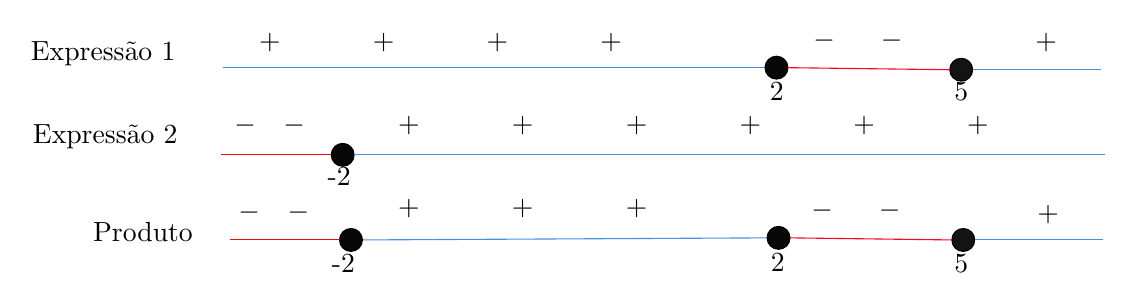
\begin{tikzpicture}[x=0.75pt,y=0.75pt,yscale=-1,xscale=1]

\draw [color={rgb, 255:red, 235; green, 11; blue, 11 }  ,draw opacity=1 ]   (101,111) -- (154,111) ;
%Shape: Circle [id:dp17867708220140965] 
\draw  [fill={rgb, 255:red, 7; green, 7; blue, 7 }  ,fill opacity=1 ] (154,111) .. controls (154,107.96) and (156.46,105.5) .. (159.5,105.5) .. controls (162.54,105.5) and (165,107.96) .. (165,111) .. controls (165,114.04) and (162.54,116.5) .. (159.5,116.5) .. controls (156.46,116.5) and (154,114.04) .. (154,111) -- cycle ;
%Straight Lines [id:da32527376127659346] 
\draw [color={rgb, 255:red, 74; green, 144; blue, 226 }  ,draw opacity=1 ]   (165,111) -- (527,111) ;
%Straight Lines [id:da9329789261744439] 
\draw [color={rgb, 255:red, 74; green, 144; blue, 226 }  ,draw opacity=1 ]   (102,69) -- (363,69) ;
%Shape: Circle [id:dp25271154714791644] 
\draw  [fill={rgb, 255:red, 8; green, 8; blue, 8 }  ,fill opacity=1 ] (363,69) .. controls (363,65.96) and (365.46,63.5) .. (368.5,63.5) .. controls (371.54,63.5) and (374,65.96) .. (374,69) .. controls (374,72.04) and (371.54,74.5) .. (368.5,74.5) .. controls (365.46,74.5) and (363,72.04) .. (363,69) -- cycle ;
%Shape: Circle [id:dp09046833829659606] 
\draw  [fill={rgb, 255:red, 20; green, 19; blue, 19 }  ,fill opacity=1 ] (452,70) .. controls (452,66.96) and (454.46,64.5) .. (457.5,64.5) .. controls (460.54,64.5) and (463,66.96) .. (463,70) .. controls (463,73.04) and (460.54,75.5) .. (457.5,75.5) .. controls (454.46,75.5) and (452,73.04) .. (452,70) -- cycle ;
%Straight Lines [id:da9967480313894097] 
\draw [color={rgb, 255:red, 247; green, 7; blue, 34 }  ,draw opacity=1 ]   (374,69) -- (452,70) ;
%Straight Lines [id:da9645451066891781] 
\draw [color={rgb, 255:red, 74; green, 144; blue, 226 }  ,draw opacity=1 ]   (463,70) -- (525,70) ;
%Straight Lines [id:da9568143770136996] 
\draw [color={rgb, 255:red, 74; green, 144; blue, 226 }  ,draw opacity=1 ]   (169,152) -- (364,151) ;
%Shape: Circle [id:dp8487660824468224] 
\draw  [fill={rgb, 255:red, 8; green, 8; blue, 8 }  ,fill opacity=1 ] (364,151) .. controls (364,147.96) and (366.46,145.5) .. (369.5,145.5) .. controls (372.54,145.5) and (375,147.96) .. (375,151) .. controls (375,154.04) and (372.54,156.5) .. (369.5,156.5) .. controls (366.46,156.5) and (364,154.04) .. (364,151) -- cycle ;
%Shape: Circle [id:dp4994180586085748] 
\draw  [fill={rgb, 255:red, 20; green, 19; blue, 19 }  ,fill opacity=1 ] (453,152) .. controls (453,148.96) and (455.46,146.5) .. (458.5,146.5) .. controls (461.54,146.5) and (464,148.96) .. (464,152) .. controls (464,155.04) and (461.54,157.5) .. (458.5,157.5) .. controls (455.46,157.5) and (453,155.04) .. (453,152) -- cycle ;
%Straight Lines [id:da24916310298444788] 
\draw [color={rgb, 255:red, 247; green, 7; blue, 34 }  ,draw opacity=1 ]   (375,151) -- (453,152) ;
%Straight Lines [id:da23935991401671264] 
\draw [color={rgb, 255:red, 74; green, 144; blue, 226 }  ,draw opacity=1 ]   (464,152) -- (526,152) ;
%Shape: Circle [id:dp7910642357859696] 
\draw  [fill={rgb, 255:red, 8; green, 8; blue, 8 }  ,fill opacity=1 ] (158,152) .. controls (158,148.96) and (160.46,146.5) .. (163.5,146.5) .. controls (166.54,146.5) and (169,148.96) .. (169,152) .. controls (169,155.04) and (166.54,157.5) .. (163.5,157.5) .. controls (160.46,157.5) and (158,155.04) .. (158,152) -- cycle ;
%Straight Lines [id:da6017888128884432] 
\draw [color={rgb, 255:red, 235; green, 11; blue, 11 }  ,draw opacity=1 ]   (105,152) -- (158,152) ;

% Text Node
\draw (151,116) node [anchor=north west][inner sep=0.75pt]   [align=left] {\mbox{-}2};
% Text Node
\draw (8,55) node [anchor=north west][inner sep=0.75pt]   [align=left] {Expressão 1};
% Text Node
\draw (38,142) node [anchor=north west][inner sep=0.75pt]   [align=left] {Produto};
% Text Node
\draw (153,158) node [anchor=north west][inner sep=0.75pt]   [align=left] {\mbox{-}2};
% Text Node
\draw (364.5,157.5) node [anchor=north west][inner sep=0.75pt]   [align=left] {2};
% Text Node
\draw (364,75) node [anchor=north west][inner sep=0.75pt]   [align=left] {2};
% Text Node
\draw (453,158) node [anchor=north west][inner sep=0.75pt]   [align=left] {5};
% Text Node
\draw (453,75) node [anchor=north west][inner sep=0.75pt]   [align=left] {5};
% Text Node
\draw (118,51) node [anchor=north west][inner sep=0.75pt]   [align=left] {$+$ \ \ \ \ \ \ \ \ \ $+$ \ \ \ \ \ \ \ \ \ $+$ \ \ \ \ \ \ \ \ \ $+$};
% Text Node
\draw (185,91) node [anchor=north west][inner sep=0.75pt]   [align=left] {$+$ \ \ \ \ \ \ \ \ \ $+$ \ \ \ \ \ \ \ \ \ $+$ \ \ \ \ \ \ \ \ \ $+$ \ \ \ \ \ \ \ \ \ $+$ \ \ \ \ \ \ \ \ \ $+$  };
% Text Node
\draw (185,131) node [anchor=north west][inner sep=0.75pt]   [align=left] {$+$ \ \ \ \ \ \ \ \ \ $+$ \ \ \ \ \ \ \ \ \ $+$};
% Text Node
\draw (493,134) node [anchor=north west][inner sep=0.75pt]   [align=left] {+ };
% Text Node
\draw (492,51) node [anchor=north west][inner sep=0.75pt]   [align=left] {+ };
% Text Node
\draw (108,133) node [anchor=north west][inner sep=0.75pt]   [align=left] {$-$ \ \ $-$};
% Text Node
\draw (384,132) node [anchor=north west][inner sep=0.75pt]   [align=left] {$-$ \ \ \ \ $-$};
% Text Node
\draw (385,50) node [anchor=north west][inner sep=0.75pt]   [align=left] {$-$ \ \ \ \ $-$ };
% Text Node
\draw (106,91) node [anchor=north west][inner sep=0.75pt]   [align=left] {$-$ \ \ $-$};
% Text Node
\draw (9,95) node [anchor=north west][inner sep=0.75pt]   [align=left] {Expressão 2};
\end{tikzpicture}
	
	Portanto, o conjunto solução final da Inequação produto é: 
	\[
	S = \{ x \in \mathbb{R} \mid -2 \le x \le 2 \; \text{ou} \; x \ge 5 \}
	\]
	
    \item Determinar o conjunto solução da inequação quociente $ \dfrac{-x^2+4x-3}{-x+2} \ge 0$\\

    \noindent
	Resolução:\\
	
	Igualando a expressão do numerador à zero, temos:\\
	$ -x^2+4x-3 = 0$\\
	Seja $a=-1, b=4, c=-3$:\\
	\[
	\Delta = b^2 - 4 \cdot a \cdot c
	\]
	\[
	\Delta = 4^2 - 4 \cdot (-1) \cdot (-3)
	\]
	\[
	\Delta = 16 - 12 = 4 > 0 \longrightarrow (x_1 \neq x_2)
	\]
	Calculando os valores das raízes
	\[
	x = \dfrac{-b \pm \sqrt{ \Delta}}{2a}
	\]
	\[
	x = \dfrac{-4 \pm \sqrt{4}}{2 \cdot (-1)}
	\]
	\[
	x = \dfrac{-4 \pm 2}{-2} 
	\]
	\[
	x_1 = \dfrac{-4 + 2}{-2} =\dfrac{-2}{-2} = 1\\
	\]
	\[
	x_2 = \dfrac{-4 - 2}{-2} =\dfrac{-6}{-2} = 3\\
	\]

            %%%%%%%%%%%%%%%%%%%%%%%%%%%%%%%%%%%%%%	
        \begin{center}
		  \begin{tikzpicture}
            \begin{axis}[
            width=0.8\textwidth,
            xlabel=$x$,
            ylabel=$y$,
            axis lines=middle,
            xmin=-2,
            xmax=6,
            ymin=-6,
            ymax=2,
            xtick={-2,1,...,6},
            ytick={-6,-5,...,2},
            enlargelimits,
            ticks=both,
            %tick label style={font=\small}, % para diminuir o tamanho de fonte
            tick label style={font=\footnotesize}, % outra opção de tamanho de fonte
            % tick label style={font=\tiny} % é a menor fonte q tem
            after end axis/.code={
            \draw (axis cs:0,\pgfkeysvalueof{/pgfplots/ymin}) -- (axis cs:0,\pgfkeysvalueof{/pgfplots/ymax});
            \draw (axis cs:\pgfkeysvalueof{/pgfplots/xmin},0) -- (axis cs:\pgfkeysvalueof{/pgfplots/xmax},0);
            \node[black, above right] at (axis cs:2,1) {$y=-x^2+4x-3$};
            }
            ]
            \addplot[domain=-2:6, blue, samples=100] {-x^2+4*x-3};
            \end{axis}
        \end{tikzpicture}
    \end{center}
            %%%%%%%%%%%%%%%%%%%%%%%%%%%%%%%%%%%%%%
 
	Igualando a expressão do denominador à zero, temos:\\
	\[ -x + 2 = 0 \]
	\[ -x = -2 \]
	\[ x = 2 \]

    
            %%%%%%%%%%%%%%%%%%%%%%%%%%%%%%%%%%%%%%	
        \begin{center}
		  \begin{tikzpicture}
            \begin{axis}[
            width=0.8\textwidth,
            xlabel=$x$,
            ylabel=$y$,
            axis lines=middle,
            xmin=-2,
            xmax=6,
            ymin=-6,
            ymax=6,
            xtick={-2,-1,...,6},
            ytick={-4,-5,...,6},
            enlargelimits,
            ticks=both,
            %tick label style={font=\small}, % para diminuir o tamanho de fonte
            tick label style={font=\footnotesize}, % outra opção de tamanho de fonte
            % tick label style={font=\tiny} % é a menor fonte q tem
            after end axis/.code={
            \draw (axis cs:0,\pgfkeysvalueof{/pgfplots/ymin}) -- (axis cs:0,\pgfkeysvalueof{/pgfplots/ymax});
            \draw (axis cs:\pgfkeysvalueof{/pgfplots/xmin},0) -- (axis cs:\pgfkeysvalueof{/pgfplots/xmax},0);
            \node[black, above right] at (axis cs:1,1.4) {$y=-x+2$};
            }
            ]
            \addplot[domain=-2:6, blue, samples=100] {-x+2};
            \end{axis}
        \end{tikzpicture}
    \end{center}
            %%%%%%%%%%%%%%%%%%%%%%%%%%%%%%%%%%%%%%
 
	Deve-se lembrar que a condição de existência da inequação é que $x \neq 2$.
	
	Estudando os sinais das soluções, temos:\\
	
	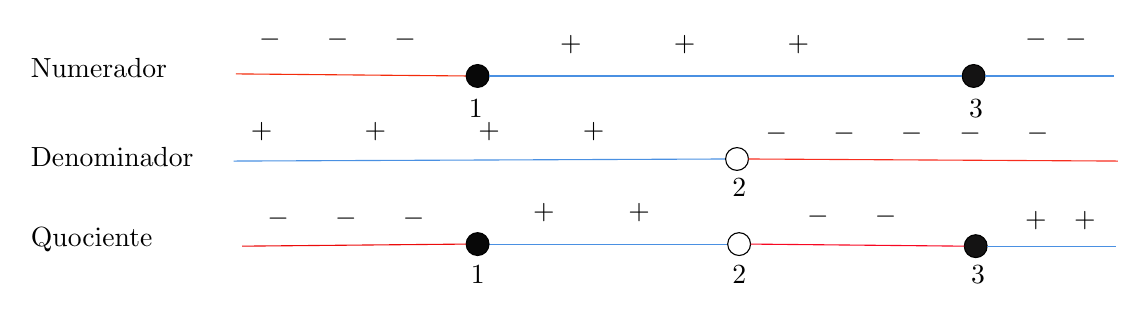
\begin{tikzpicture}[x=0.75pt,y=0.75pt,yscale=-1,xscale=1]
		\draw [color={rgb, 255:red, 74; green, 144; blue, 226 }  ,draw opacity=1 ]   (101,111) -- (338,110) ;
		\draw  [fill={rgb, 255:red, 255; green, 255; blue, 255 }  ,fill opacity=1 ] (338,110) .. controls (338,106.96) and (340.46,104.5) .. (343.5,104.5) .. controls (346.54,104.5) and (349,106.96) .. (349,110) .. controls (349,113.04) and (346.54,115.5) .. (343.5,115.5) .. controls (340.46,115.5) and (338,113.04) .. (338,110) -- cycle ;
		\draw [color={rgb, 255:red, 247; green, 45; blue, 30 }  ,draw opacity=1 ]   (349,110) -- (527,111) ;
		\draw [color={rgb, 255:red, 243; green, 43; blue, 11 }  ,draw opacity=1 ]   (102,69) -- (213,70) ;
		\draw  [fill={rgb, 255:red, 8; green, 8; blue, 8 }  ,fill opacity=1 ] (213,70) .. controls (213,66.96) and (215.46,64.5) .. (218.5,64.5) .. controls (221.54,64.5) and (224,66.96) .. (224,70) .. controls (224,73.04) and (221.54,75.5) .. (218.5,75.5) .. controls (215.46,75.5) and (213,73.04) .. (213,70) -- cycle ;
		\draw  [fill={rgb, 255:red, 20; green, 19; blue, 19 }  ,fill opacity=1 ] (452,70) .. controls (452,66.96) and (454.46,64.5) .. (457.5,64.5) .. controls (460.54,64.5) and (463,66.96) .. (463,70) .. controls (463,73.04) and (460.54,75.5) .. (457.5,75.5) .. controls (454.46,75.5) and (452,73.04) .. (452,70) -- cycle ;
		\draw [color={rgb, 255:red, 74; green, 144; blue, 226 }  ,draw opacity=1 ]   (224,70) -- (452,70) ;
		\draw [color={rgb, 255:red, 74; green, 144; blue, 226 }  ,draw opacity=1 ]   (463,70) -- (525,70) ;
		\draw [color={rgb, 255:red, 74; green, 144; blue, 226 }  ,draw opacity=1 ]   (224,151) -- (339,151) ;
		\draw  [fill={rgb, 255:red, 255; green, 255; blue, 255 }  ,fill opacity=1 ] (339,151) .. controls (339,147.96) and (341.46,145.5) .. (344.5,145.5) .. controls (347.54,145.5) and (350,147.96) .. (350,151) .. controls (350,154.04) and (347.54,156.5) .. (344.5,156.5) .. controls (341.46,156.5) and (339,154.04) .. (339,151) -- cycle ;
		\draw  [fill={rgb, 255:red, 20; green, 19; blue, 19 }  ,fill opacity=1 ] (453,152) .. controls (453,148.96) and (455.46,146.5) .. (458.5,146.5) .. controls (461.54,146.5) and (464,148.96) .. (464,152) .. controls (464,155.04) and (461.54,157.5) .. (458.5,157.5) .. controls (455.46,157.5) and (453,155.04) .. (453,152) -- cycle ;
		\draw [color={rgb, 255:red, 247; green, 7; blue, 34 }  ,draw opacity=1 ]   (350,151) -- (453,152) ;
		\draw [color={rgb, 255:red, 74; green, 144; blue, 226 }  ,draw opacity=1 ]   (464,152) -- (526,152) ;
		\draw  [fill={rgb, 255:red, 8; green, 8; blue, 8 }  ,fill opacity=1 ] (213,151) .. controls (213,147.96) and (215.46,145.5) .. (218.5,145.5) .. controls (221.54,145.5) and (224,147.96) .. (224,151) .. controls (224,154.04) and (221.54,156.5) .. (218.5,156.5) .. controls (215.46,156.5) and (213,154.04) .. (213,151) -- cycle ;
		\draw [color={rgb, 255:red, 235; green, 11; blue, 11 }  ,draw opacity=1 ]   (105,152) -- (213,151) ;
		\draw (2,60) node [anchor=north west][inner sep=0.75pt]   [align=left] {Numerador};
		\draw (2,103) node [anchor=north west][inner sep=0.75pt]   [align=left] {Denominador};
		\draw (2,142) node [anchor=north west][inner sep=0.75pt]   [align=left] {Quociente};
		\draw (214,160) node [anchor=north west][inner sep=0.75pt]   [align=left] {1};
		\draw (340,160) node [anchor=north west][inner sep=0.75pt]   [align=left] {2};
		\draw (213,80) node [anchor=north west][inner sep=0.75pt]   [align=left] {1};
		\draw (455,160) node [anchor=north west][inner sep=0.75pt]   [align=left] {3};
		\draw (454,80) node [anchor=north west][inner sep=0.75pt]   [align=left] {3};
		\draw (257,49) node [anchor=north west][inner sep=0.75pt]   [align=left] {$+$ \ \ \ \ \ \ \ \ \ $+$ \ \ \ \ \ \ \ \ \ $+$ };
		\draw (108,91) node [anchor=north west][inner sep=0.75pt]   [align=left] {$+$ \ \ \ \ \ \ \ \ \ $+$ \ \ \ \ \ \ \ \ \ $+$\ \ \ \ \ \ \ \ \ $+$ };
		\draw (244,130) node [anchor=north west][inner sep=0.75pt]   [align=left] { $+$ \ \ \ \ \ \ \ $+$ \ };
		\draw (481,134) node [anchor=north west][inner sep=0.75pt]   [align=left] {$+$\ \ \ $+$};
		\draw (481,47) node [anchor=north west][inner sep=0.75pt]   [align=left] {\mbox{$-$}\ \ $-$ };
		\draw (116,133) node [anchor=north west][inner sep=0.75pt]   [align=left] {\mbox{$-$} \ \ \ \ $-$ \ \ \ \ $-$};
		\draw (376,132) node [anchor=north west][inner sep=0.75pt]   [align=left] {\mbox{$-$} \ \ \ \ $-$};
		\draw (112,47) node [anchor=north west][inner sep=0.75pt]   [align=left] {\mbox{$-$} \ \ \ \ $-$ \ \ \ \ $-$};
		\draw (356,92) node [anchor=north west][inner sep=0.75pt]   [align=left] {\mbox{$-$} \ \ \ \ $-$ \ \ \ \ $-$\ \ \ \ $-$ \ \ \ \ $-$};
		\draw (340,118) node [anchor=north west][inner sep=0.75pt]   [align=left] {2};
	\end{tikzpicture}
	
	Portanto, o conjunto solução final da Inequação produto é: 
	\[
	S = \{ x \in \mathbb{R} \mid 1 \le x < 2 \; \text{ou} \; x \ge 3 \}
	\]

    \end{enumerate}